\documentclass[9pt,twoside,lineno]{pnas-SI}
% Use the lineno option to display guide line numbers if required.

\templatetype{pnassupportinginfo}

\title{Quantitative, Multispecies Monitoring at a Continental Scale}
\author{Gledis Guri, Owen Liu, Ryan P. Kelly, Megan Shaffer, Kim Parsons, Ana Ram\'on-Laca,\\
Krista M. Nichols, Pedro F. P. Brandão-Dias, Abigail Wells and Andrew Olaf Shelton}
\correspondingauthor{Gledis Guri.\\E-mail: gguri@uw.edu}

\begin{document}

\maketitle

%% Adds the main heading for the SI text. Comment out this line if you do not have any supporting information text.
\SItext

\section*{Extended Methods}
\subsection*{qPCR}
Environmental samples were analyzed in triplicate using the multiplexed assay targeting Pacific hake, Eulachon and Pacific lamprey as described in \cite{ramon-laca2021} on a QuanStudio 6 (Applied Biosystems). Only Pacific hake qPCR data was used in this study due to the remaining qPCR targets having little positive amplification. 

The samples underwent real-time thermocycler protocol including an initial denaturation step at 95°C 10 min followed by 45 cycles of 15 s at 95°C and 1 min at 60°C. All samples were run in triplicate in 10 $\mu$L volume consisting of 1 x TaqPath ProAmp Multiplex Master Mix, 0.9 $\mu$M of each primer (forward: AAATGTTTAAACTAGAGCCGAATAGC and reverse: TCGTGGAGTCAAAGTGGGGTAGA), 0.2 $\mu$M of probe (6FAM-CACTCGAGGCCACGAAGTACAATT-(MGB)NFQ), and 2 $\mu$L of DNA template or water for the non-template control. All reactions included 100 copies of internal positive control (IPC) to detect PCR inhibition. Any IPC delay exceeding 0.5 cycles in the non-template control was considered inhibition and inhibited samples were diluted and re-analyzed. 

Alongside environmental samples standard samples were analyzed constructed from a 130 bp synthetic DNA fragment (gBlock; IDT) representing the 12S region of Pacific hake (\textit{Merluccius productus}), which encompasses the 101 bp 12S qPCR target (sequence information available in \cite{ramon-laca2021}). The synthetic DNA fragment was diluted to create a series of standards with final concentrations ranging from $10^{0}$ to $10^{5}$ copies/$\mu$L.

\subsection*{Metabarcoding}
In total, 568 samples, including 554 environmental samples, 7 PCR blanks and 7 positive controls (holding only kangaroo DNA) were amplified using MiFish-U universal primers \cite{miya2015} with Illumina tails (forward TCGTCGGCAGCGTCAGATGTGTATAAGAGACAGGCCGGTAAAACTCGTGCCAGC; reverse GTCTCGTGGGCTCGGAGATGTGTATAAGAGACAGCATAGTGGGGTATCTAATCCCAGTTTG) by using a two-step PCR protocol. The DNA was amplified in the first PCR reaction (PCR1) in a 20 µL reaction consisting of: 10 µL of Phusion Master Mix (2X), 0.4 µL of the forward primer (10 µM); 0.4 µL of the reverse primer (10 µM), 0.6 µL of 100\% DMSO, 0.5 µL of rAlbumin (20 µg/µL), 4.4 µL of nuclease-free water and 2 µL of DNA template. Reactions were run with the following cycling conditions: an initial denaturation of 98°C for 30 sec; followed by 35 cycles of 98°C for 10 sec, 60°C for 30 sec, and of 72°C for 3 sec; with a final extension of 72°C for 10 min and hold at 4°C. 

PCR product was cleaned using Ampure Beads (1.2x) and then indexed in a second PCR reaction (PCR2), with the following recipe: 12.5 $\mu$L of KAPA HiFi HotStart ReadyMix (Roche Diagnostics), 1.25 $\mu$L of an index from IDT for Illumina DNA/RNA UD Indexes (Sets A-D), 5 $\mu$L of PCR1 product, and 6.25 $\mu$L of nuclease free water. Cycling conditions included an initial denaturation of 95°C for 5 min; 8 cycles of: 98°C for 20 sec, 56°C for 30 sec, 72°C for 1 min; and a final extension of 72°C for 5 min. Resulting products were visualized on a 2\% agarose gel and quantified using Quant-iT™ dsDNA Assay Kit (Thermo Fisher Scientific, USA) with Fluoroskan™ Microplate Fluorometer (Thermo Fisher Scientific, USA). Indexed products were normalized by concentration, pooled into libraries for sequencing, and then size- selected to extract only the target fish band using the E-Gel™ SizeSelect™ II Agarose Gels (Thermo Fisher Scientific, USA).  Subsequently the libraries were sequenced on Illumina MiSeq platform using the v3 600 cycle kit. 


\subsection*{Mock community}

We constructed mock communities with even and skewed species total genomic DNA using Qubit HS assay quantification method. We then quantified the concentration of the 12S rRNA gene using MarVer1 primers (forward: CGTGCCAGCCACCGCG; reverse: GGGTATCTAATCCYAGTTTG \cite{valsecchi2020}), which perfectly matched the template to give unbiased estimates of concentration, using ddPCR (Bio-Rad, Inc., QX200 Droplet Digital PCR system). Each tissue of each species was quantified in a 22 $\mu$L reaction consisted of 2 $\mu$L of DNA template from genomic DNA , 11 $\mu$L of ddPCR EvaGreen (Bio-Rad), 0.22 $\mu$L of each forward and reverse primers (10 uM), and 0.56 $\mu$L of nuclease free water. The thermocycler reactions were run in C1000 Touch Thermal Cycler with 96-Deep Well Reaction Module (Bio-Rad) using the PCR program as follows: 2 min at 50°C for enzyme activation, 2 min at 95°C for initial denaturation, and 40 cycles of denaturation for 1 sec at 95°C and primer annealing and elongation for 30 sec min at 60°C, with a ramp rate of 2°C per s and heldat 4°C until droplets were read. Droplets were determined to be positive after drawing a threshold based on NTCs.

\subsection*{Bioinformatics}
Starting with Illumina-demultiplexed sequencing files, we first removed primer and adapter sequences using Cutadapt v4.9, applying the default mismatch tolerance parameter (-e 0.1) \cite{martin2011}. Next, we performed quality filtering using the filterAndTrim function from the dada2 R package, retaining its default parameters while specifying the optional truncLen argument to match the minimum MiFish amplicon length. After filtering, we denoised the sequences using dada2 with default settings \cite{callahan2016}, which resulted in a list of Amplicon Sequence Variants (ASVs) across all samples. Each resulting ASV was then assigned a unique 28-character hash code using the sha-1 algorithm with the R function map\_chr. This allowed us to create a common database of ASVs by hash, enabling us to track which sequences have already been annotated for consistency and to avoid redundant computational efforts.

For taxonomic assignment of ASVs, we used standalone BLAST \cite{altschul1990} to compare each unique ASV against the NCBI nr eukaryote database as of January 2025. BLAST arguments were as follows: "-word\_size 30 -evalue "1e-30" -max\_target\_seqs 50". To streamline annotation, we also used the "-negative\_taxids" argument, including a list of target organisms closely related to those present in the sampled region, but known to be absent. The complete list of taxids that were excluded is available alongside the pipeline code. Finally, we performed a least common ancestor (LCA) analysis on the top BLAST hits using TaxonKit v0.17 \cite{shen2021}. Sequences with a 100 percent identity match to any database sequence were prioritized for LCA. In the absence of perfect matches, we conducted LCA analysis on the top hits with identity scores above 99.3, , 98, or 96 percent respectively. In the absence of any hits above 96 identity, taxonomic assignment was truncated. Finally, for mock communities were identify of species was known, we manually curated annotations before analysis. 

\subsection*{Bayesian model}
OLE

The above statistical model provides predictions of species-specific DNA concentrations (D) at each depth sampled (d = 0, 50, 150, 300 or 500 m). We used the sdmTMB package \cite{anderson2022} to generate distribution models for the concentration of eDNA , as:
$$\ln D_{xyz} = \tau + \eta(s) + \varepsilon_{d}(s)$$
where x,y,z index longitude, latitude, and depth, respectively, $\tau$ is scalar intercept, $\eta(s)$ is a spatial smooth shared among depths, and $\varepsilon_d(s)$ is a depth-specific spatial smooth. Both $\eta(s)$ and $\varepsilon_d(s)$ are a zero-centered Gaussian random field estimated using the stochastic partial differntial equation (SPDE) approximation (see \cite{anderson2022}). Each species was fitted individually while we created and selected the best mesh for approximating spatial Gaussian random fields as part of the model.

\subsection*{Model convergance}
OLE + GLED


%%% Each figure should be on its own page
\begin{figure}
\centering
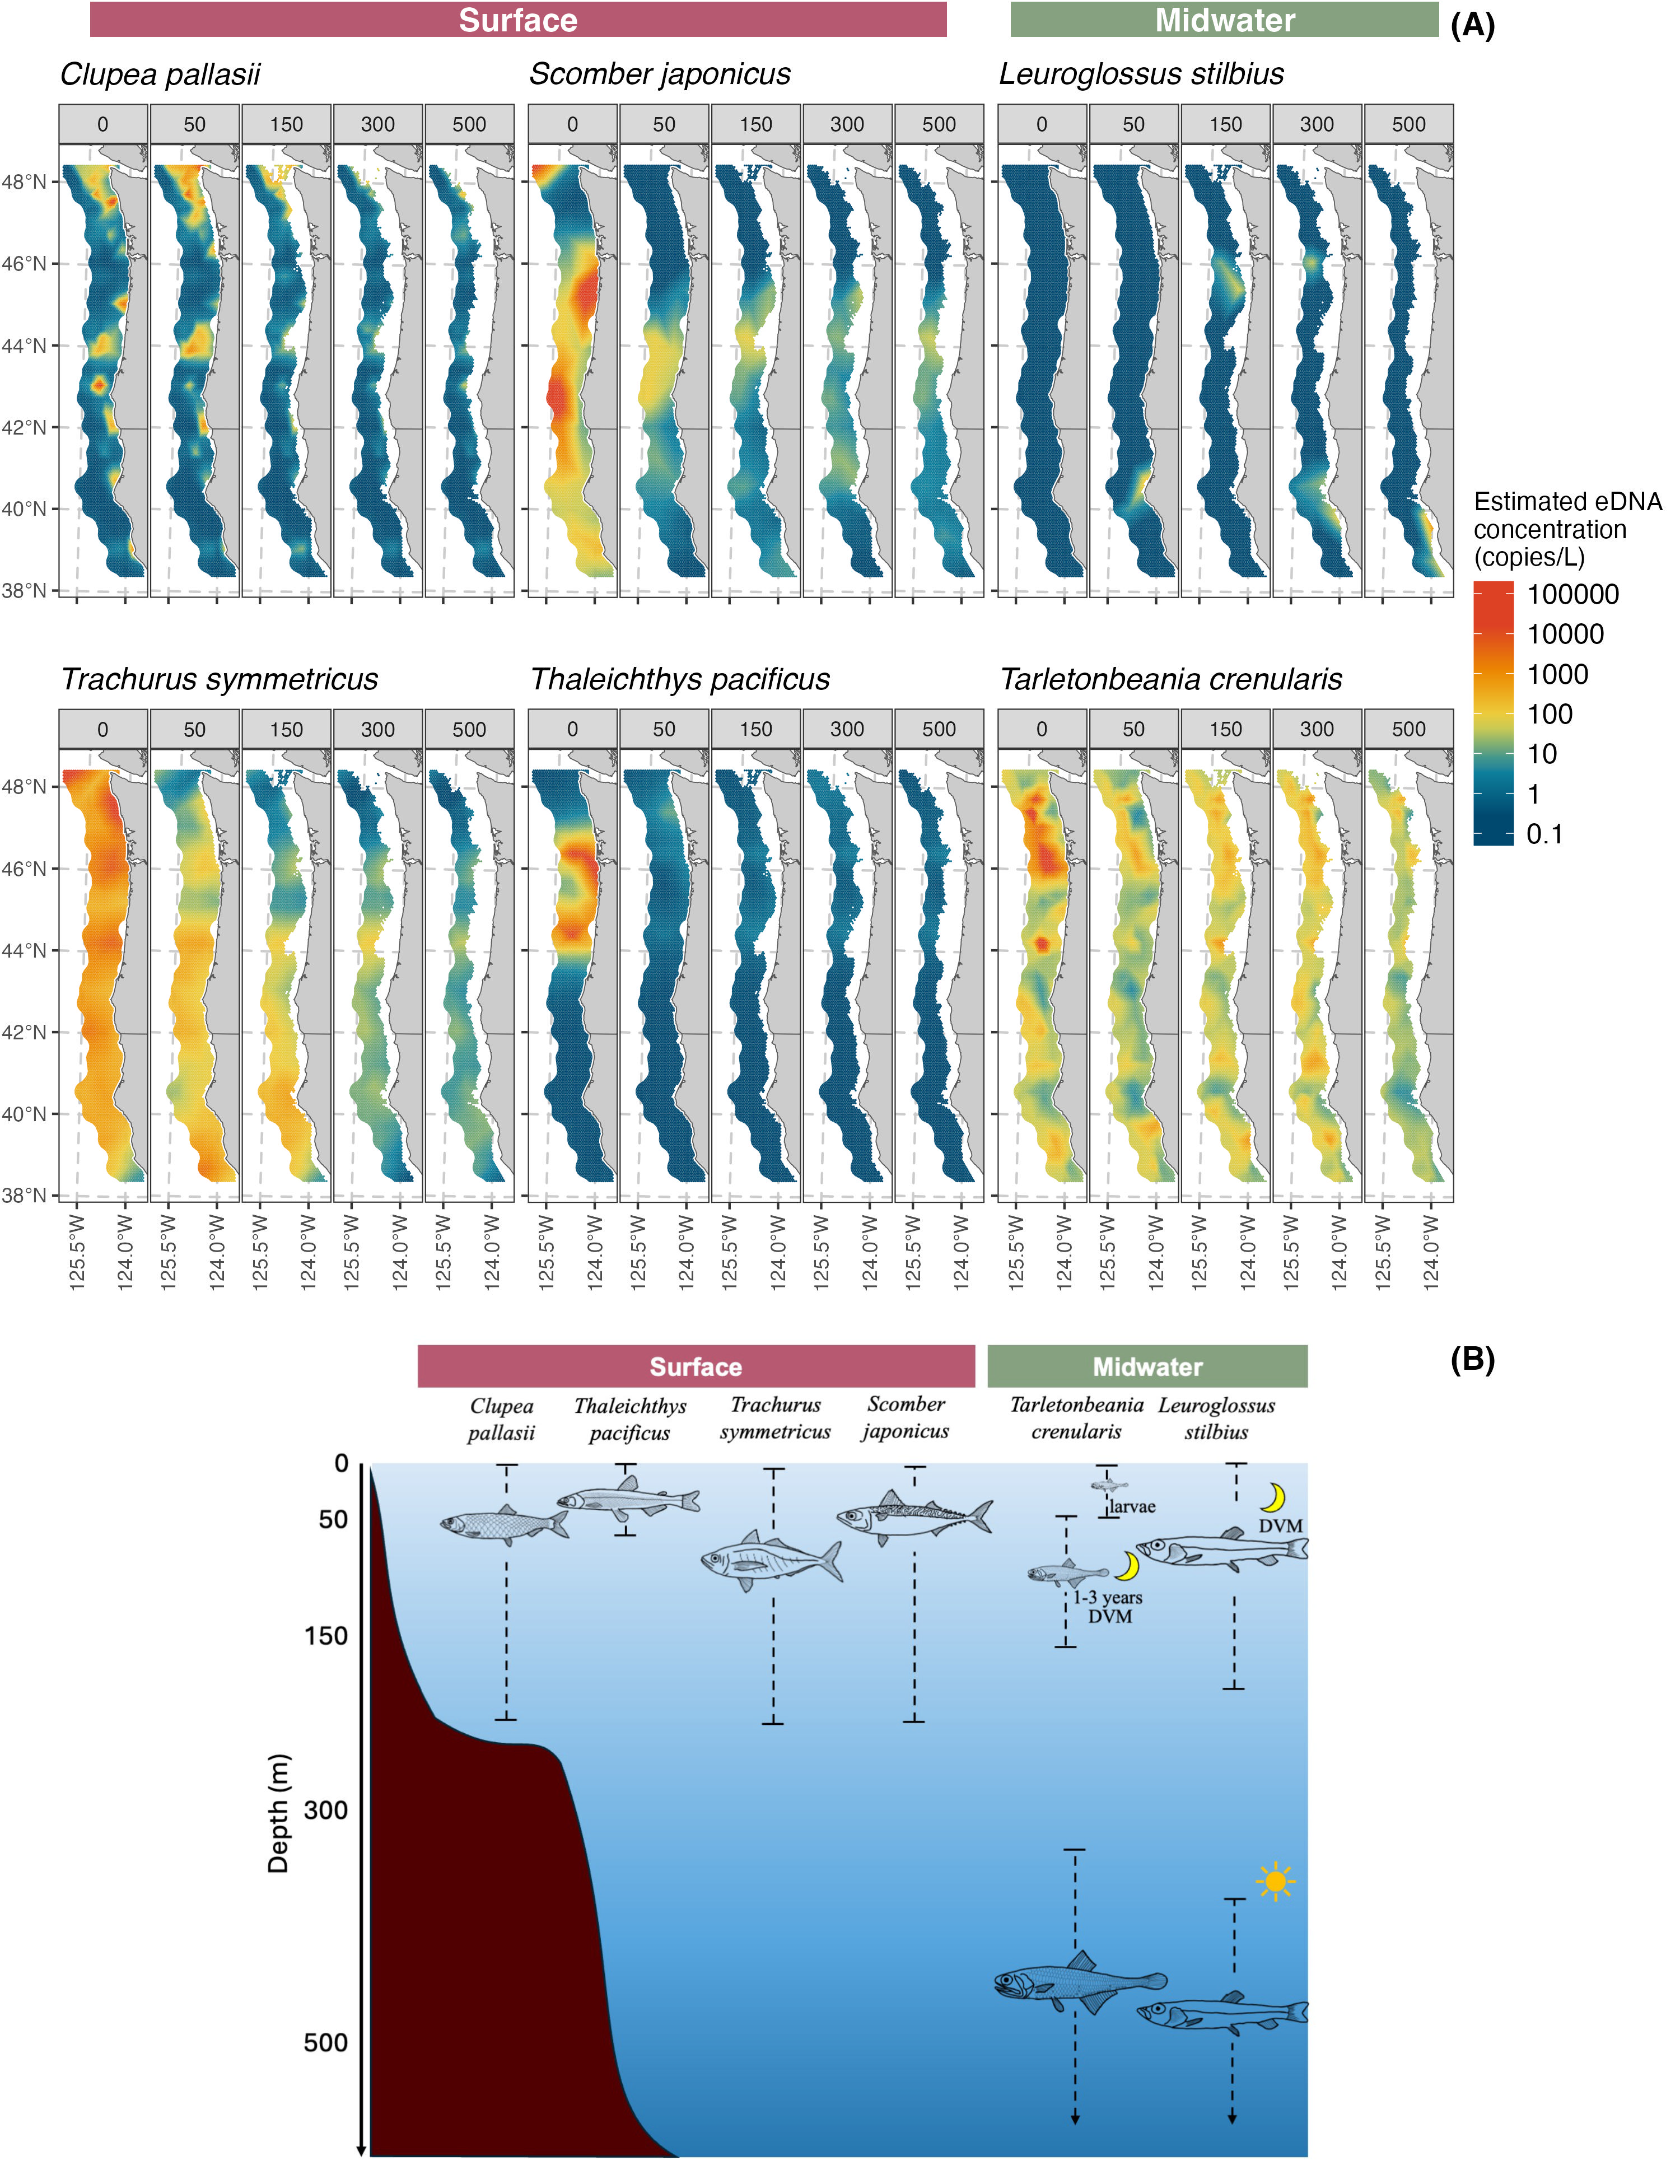
\includegraphics[width=0.98\textwidth]{plots/5_Supplementary_Figure_1.jpg}
\caption{Continuation of Fig. 1. Estimated species eDNA for \textit{Clupea pallasi}, \textit{Trachurus symmetricus}, \textit{Scomber japonicus}, \textit{Thaleichthys pacificus}, \textit{Leuroglossus stilbius}, and \textit{Tarletonbaeania crenularis} concentration (A) across 0, 50, 150, 300, and 500m depth samples and known depth distribution of those species from literature (B).}
\end{figure}

%%% Each figure should be on its own page
\begin{figure}
\centering
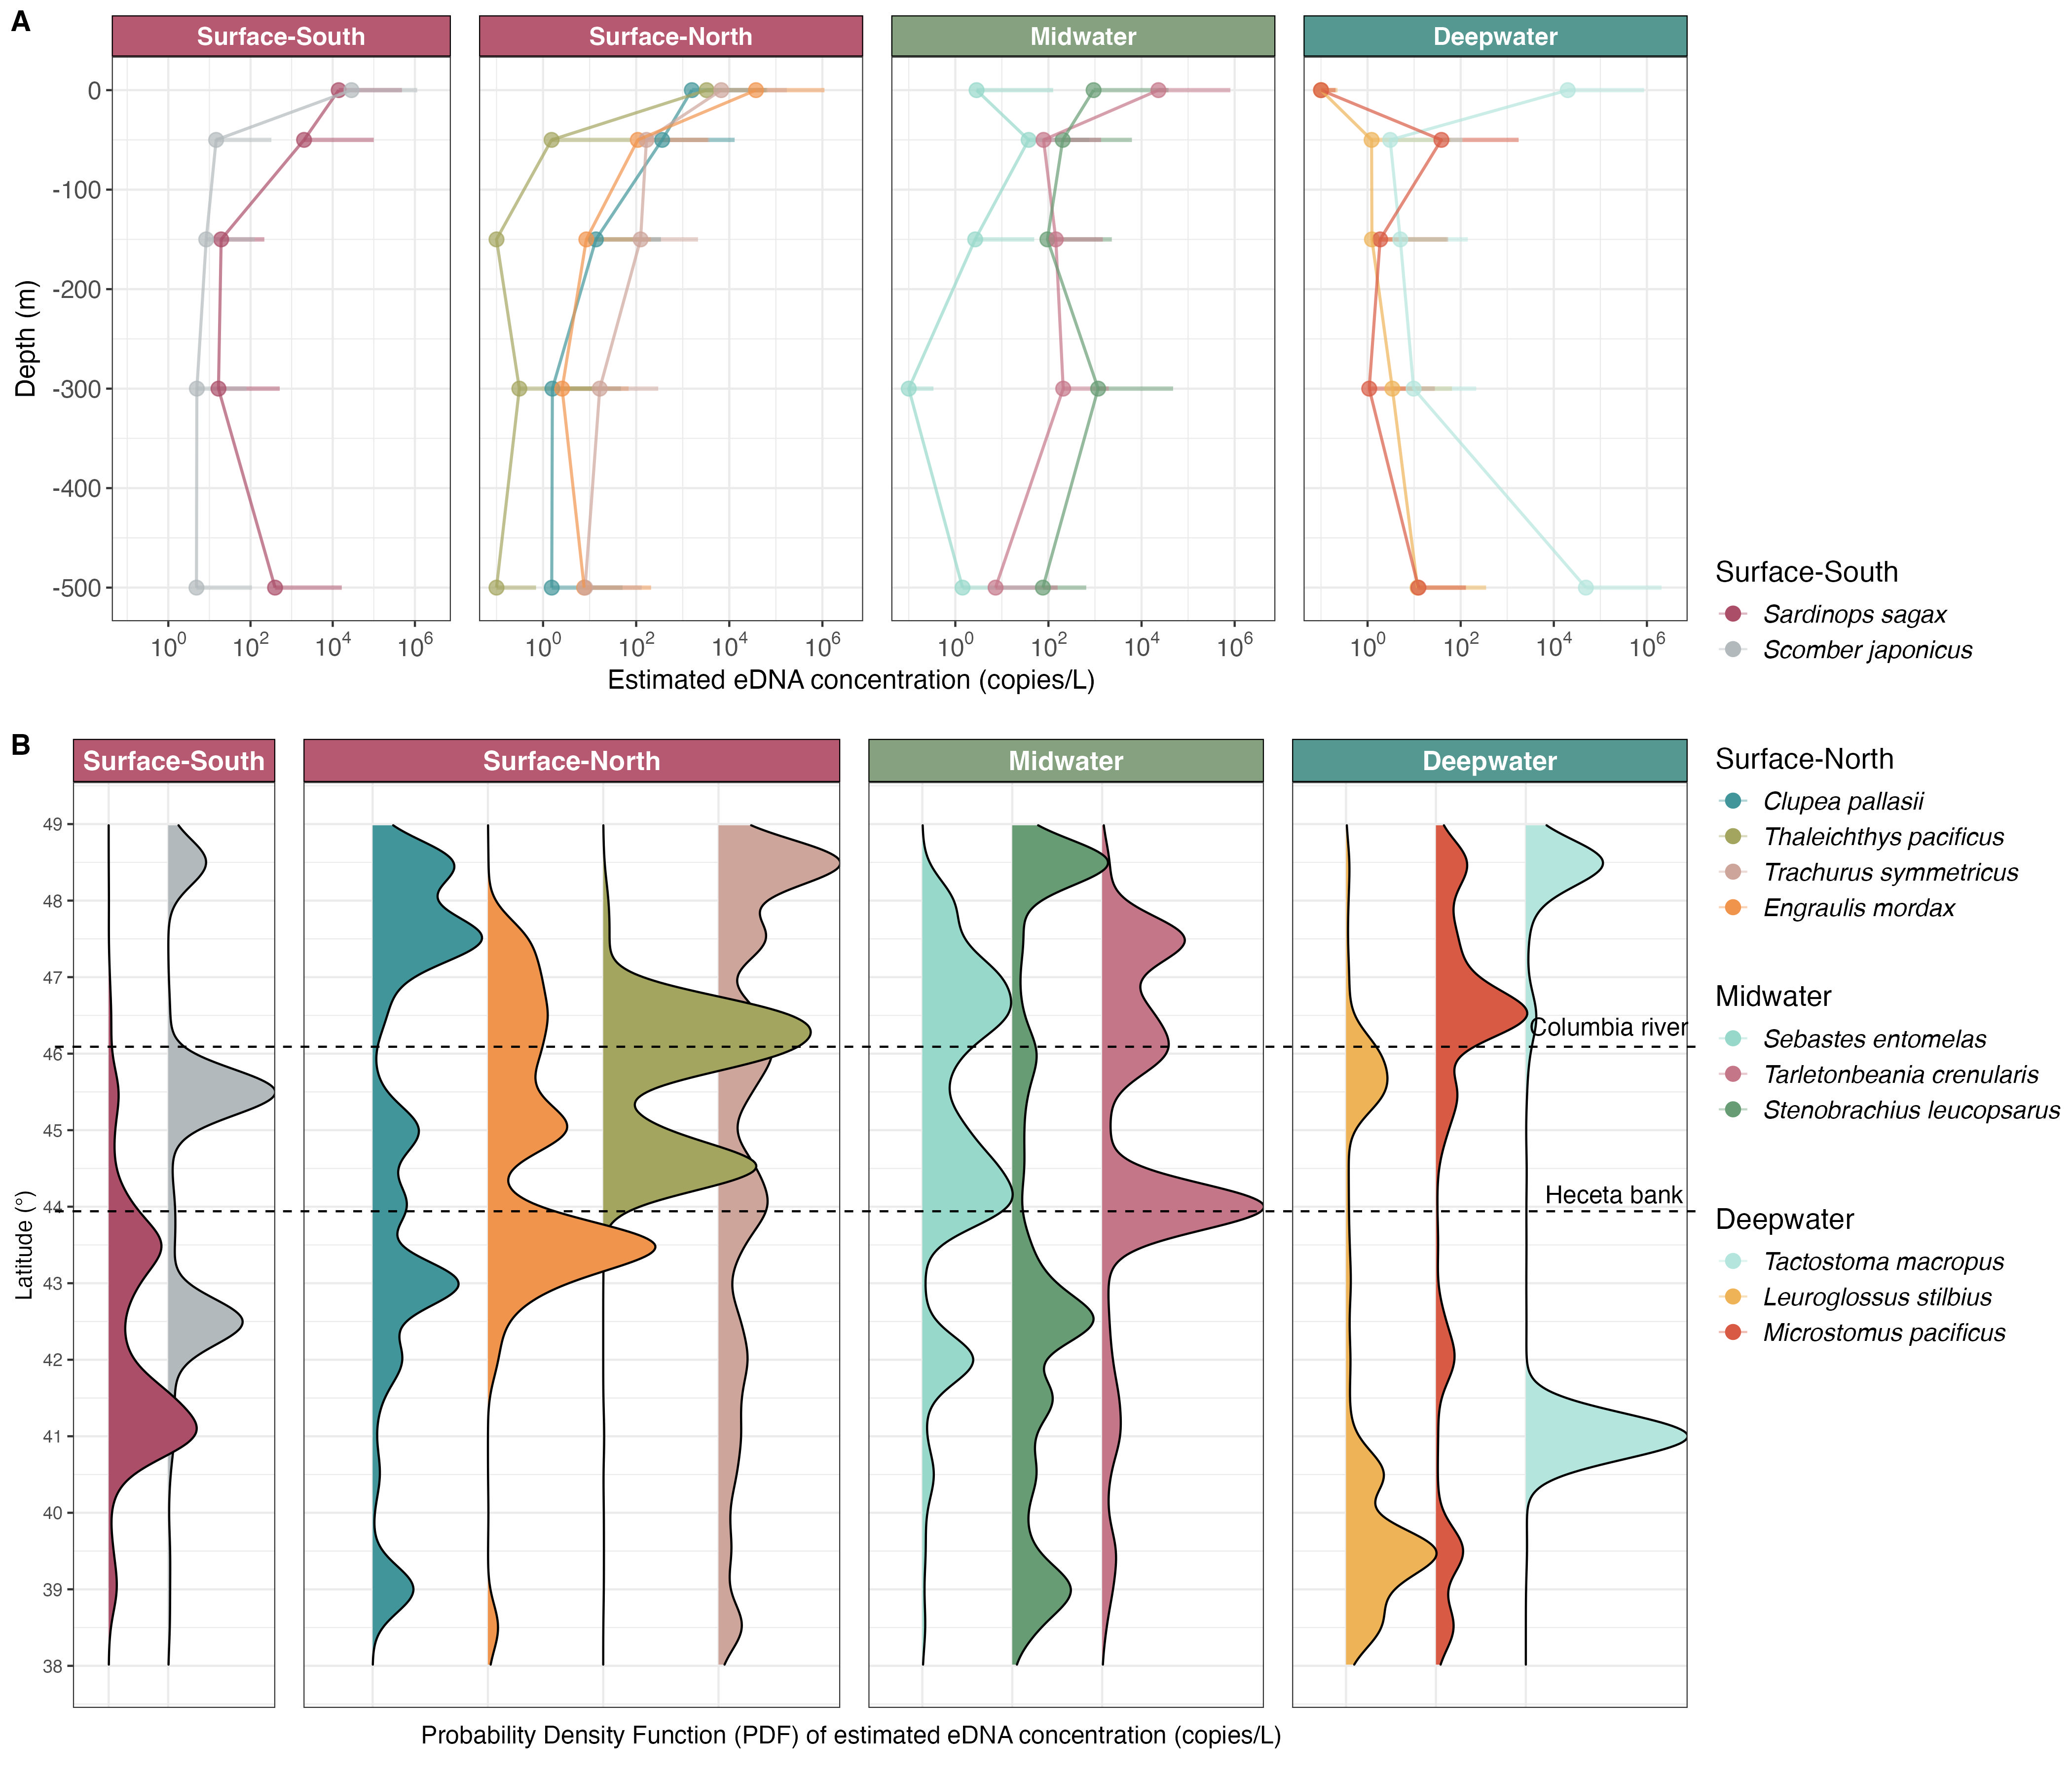
\includegraphics[width=0.89\textwidth]{plots/4_Figure_4.jpg}
\caption{Vertical (A) and latitudinal (B) distribution of eDNA concentrations grouped in ecological groups (surface south, surface north, midwater, and deepwater). Mean eDNA concentration of vertical distribution is shown with dots and 99\% upper quantile with ticks (A). Probability density functions (PDF) of estimated eDNA concentrations across latitudinal gradients (B; square root transformed of x-axis to enhance low concentration peaks). Key geographic features, such as the Columbia River and Heceta Bank, are marked to indicate alignment of species distributions.}
\end{figure}

%%% Each figure should be on its own page
\begin{figure}
\centering
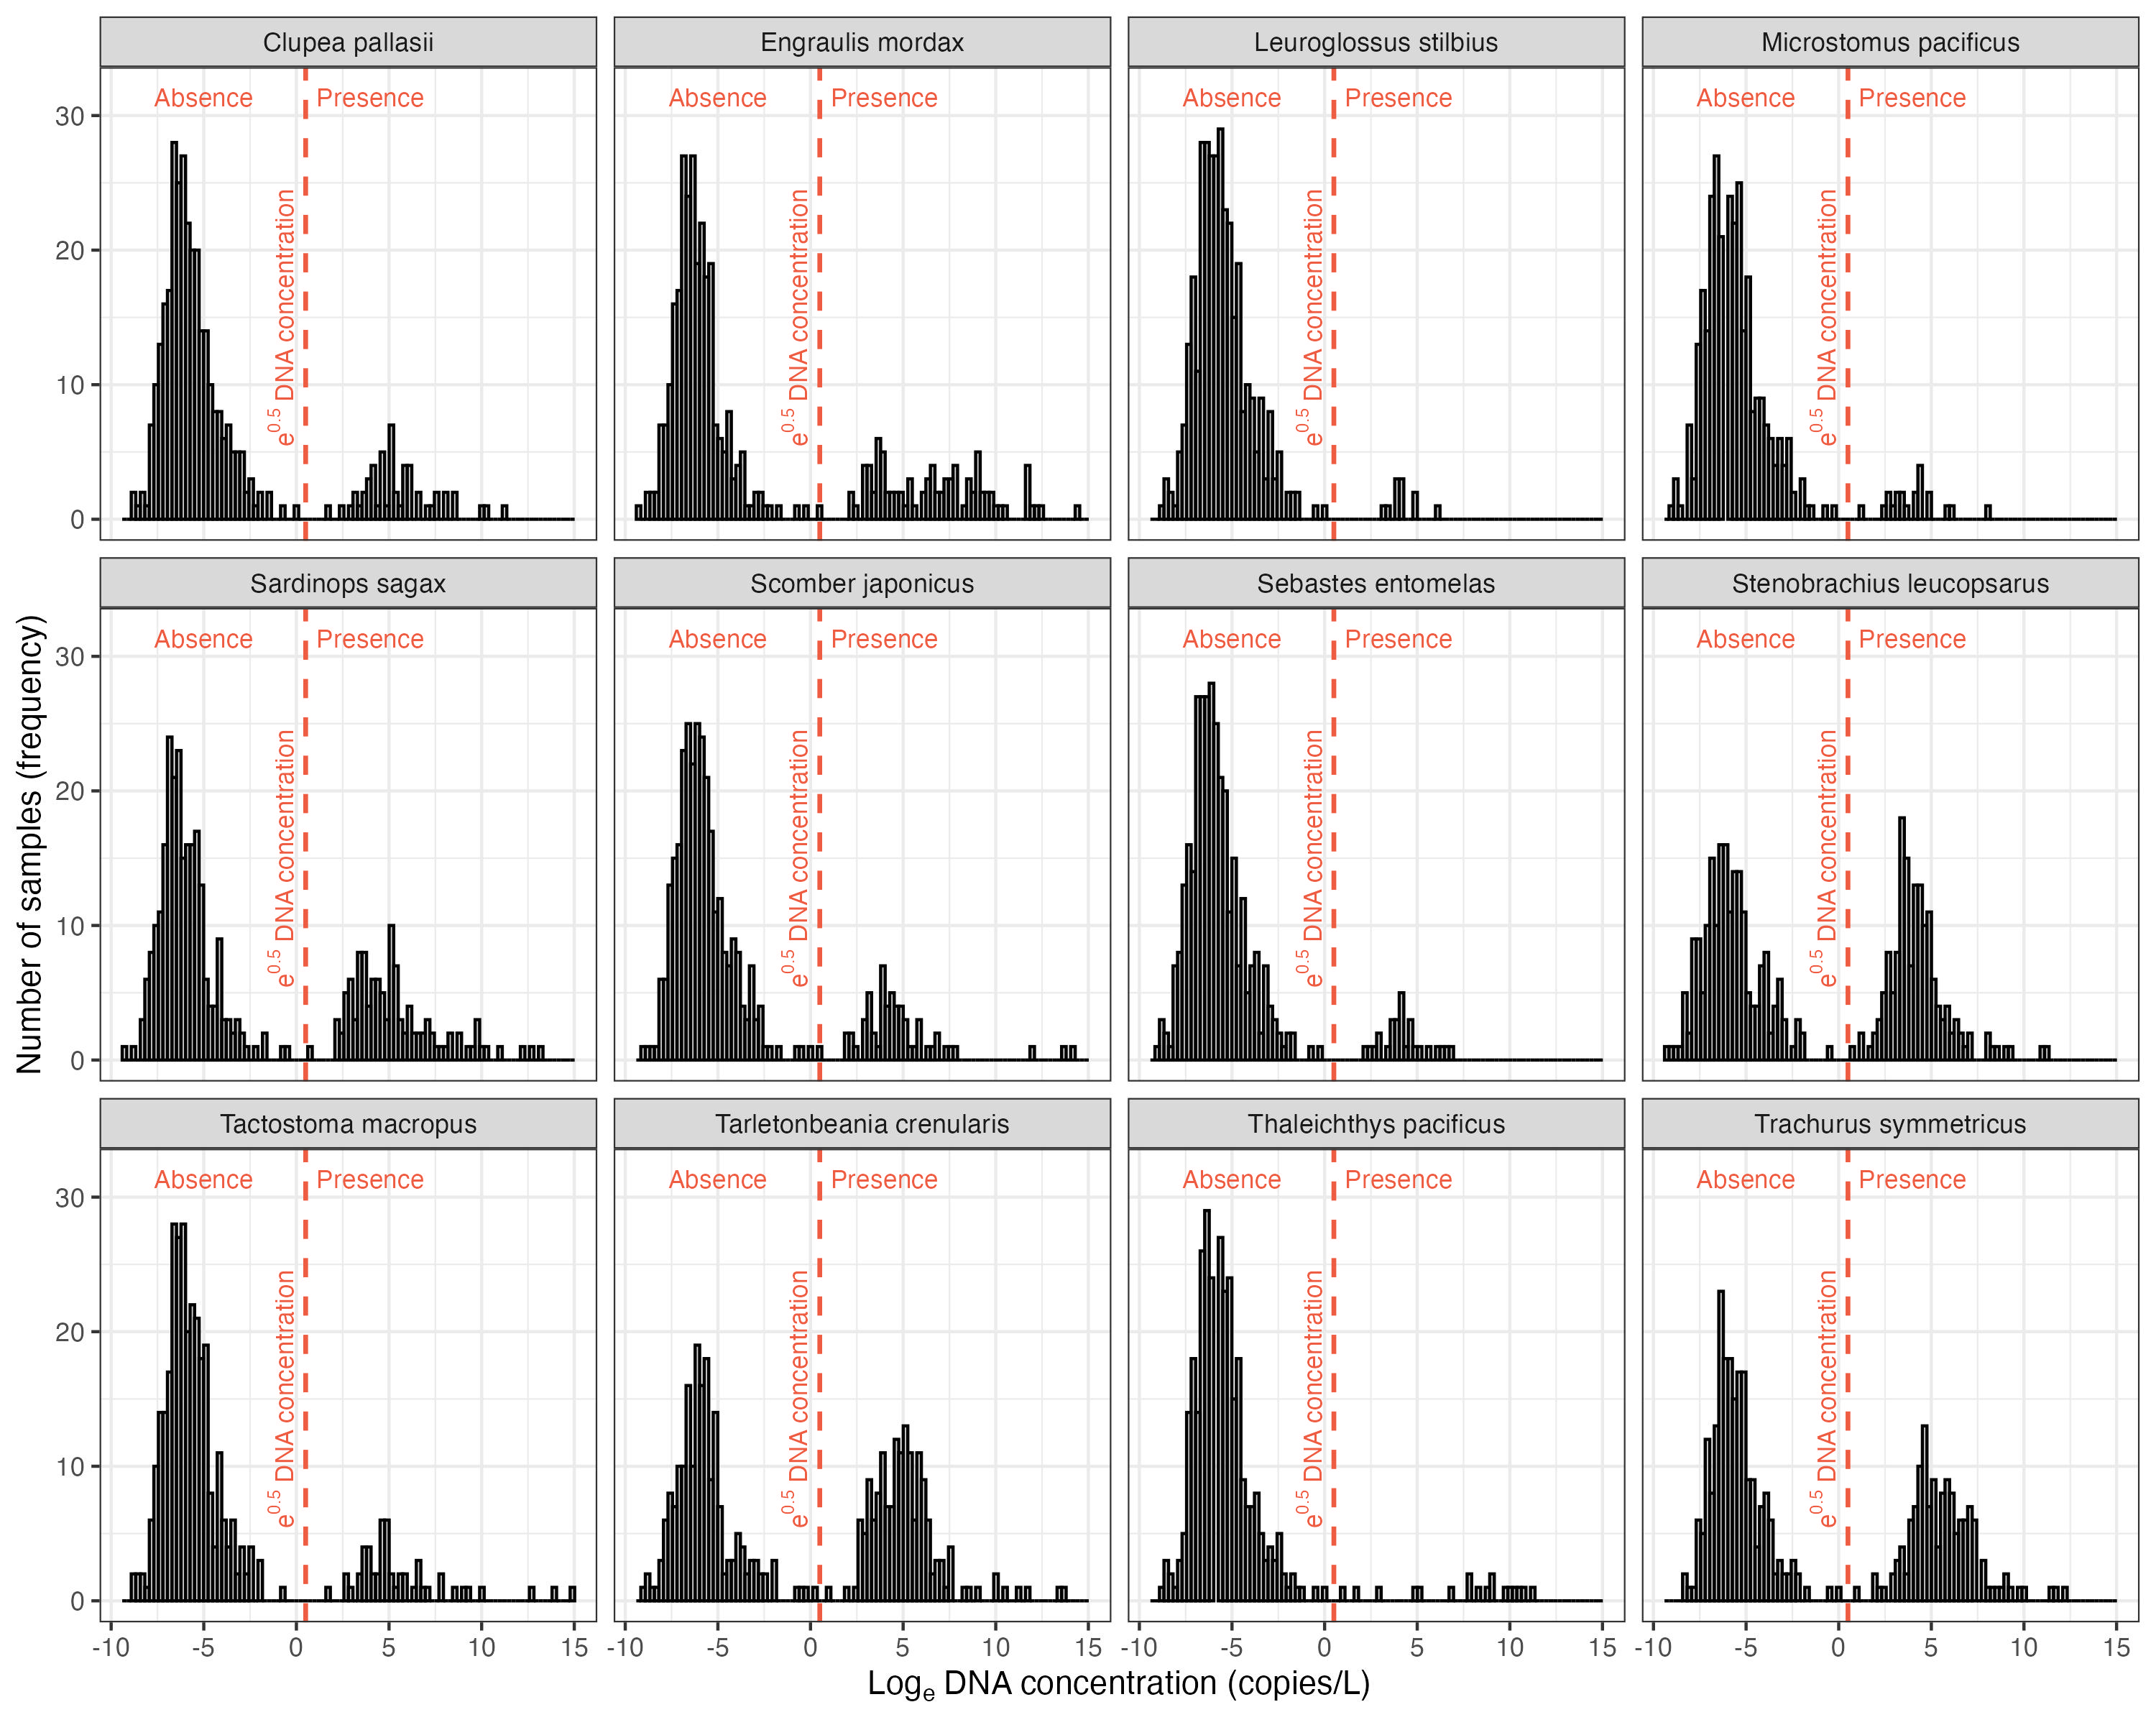
\includegraphics[width=0.99\textwidth]{plots/6_Supplementary_Figure_2.jpg}
\caption{Frequency distribution of eDNA concentration for each species included in this study (n = 12). The dashed red line indicates the threshold model estimated concentration (copies/L) for defining presence and absence of sequenced (through metabarcoding) taxa}
\end{figure}

%%% Each figure should be on its own page
\begin{figure}
\centering
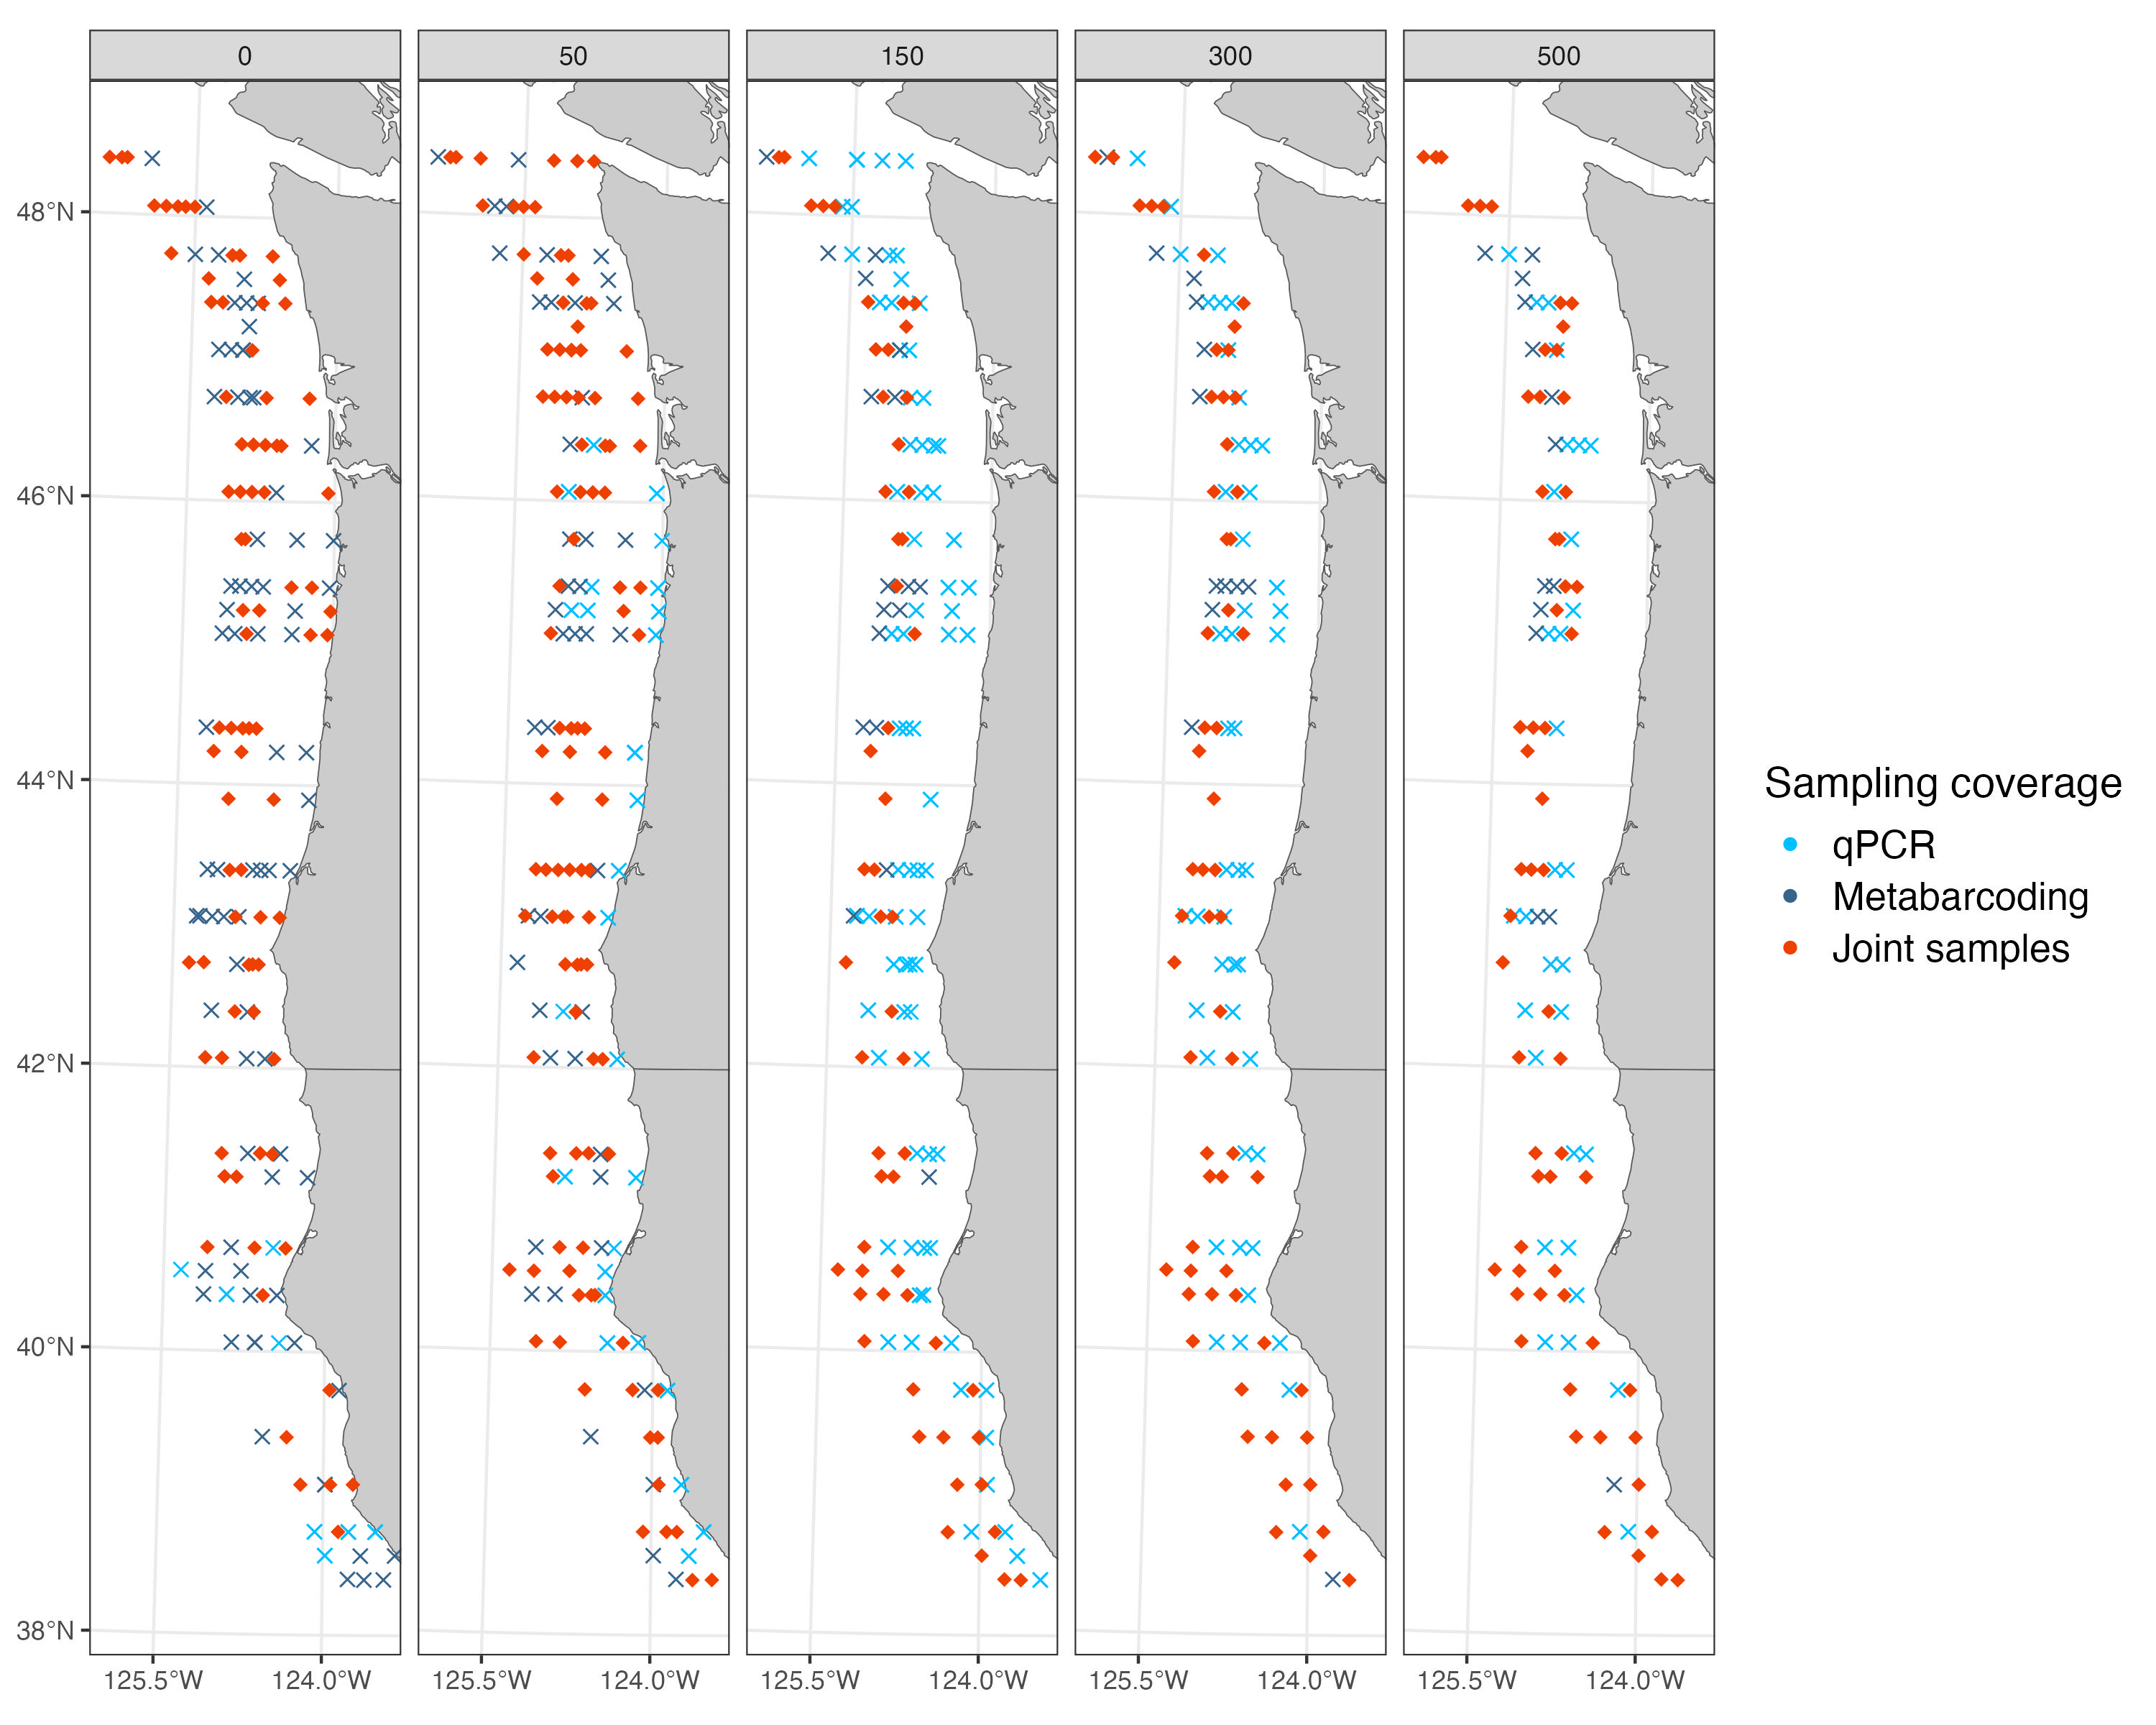
\includegraphics[width=0.99\textwidth]{plots/7_Supplementary_Figure_3.jpg}
\caption{Three-dimensional distribution of samples collected that were run through qPCR (light blue), metabarcoding (dark blue), and were used jointly in the Bayesian model (Fig. 4; red). Jointly modeled samples are those that detected Pacific hake -- used as a reference species for quantification -- in both qPCR and metabarcoding assays.}
\end{figure}

%%% Each figure should be on its own page
\begin{figure}
\centering
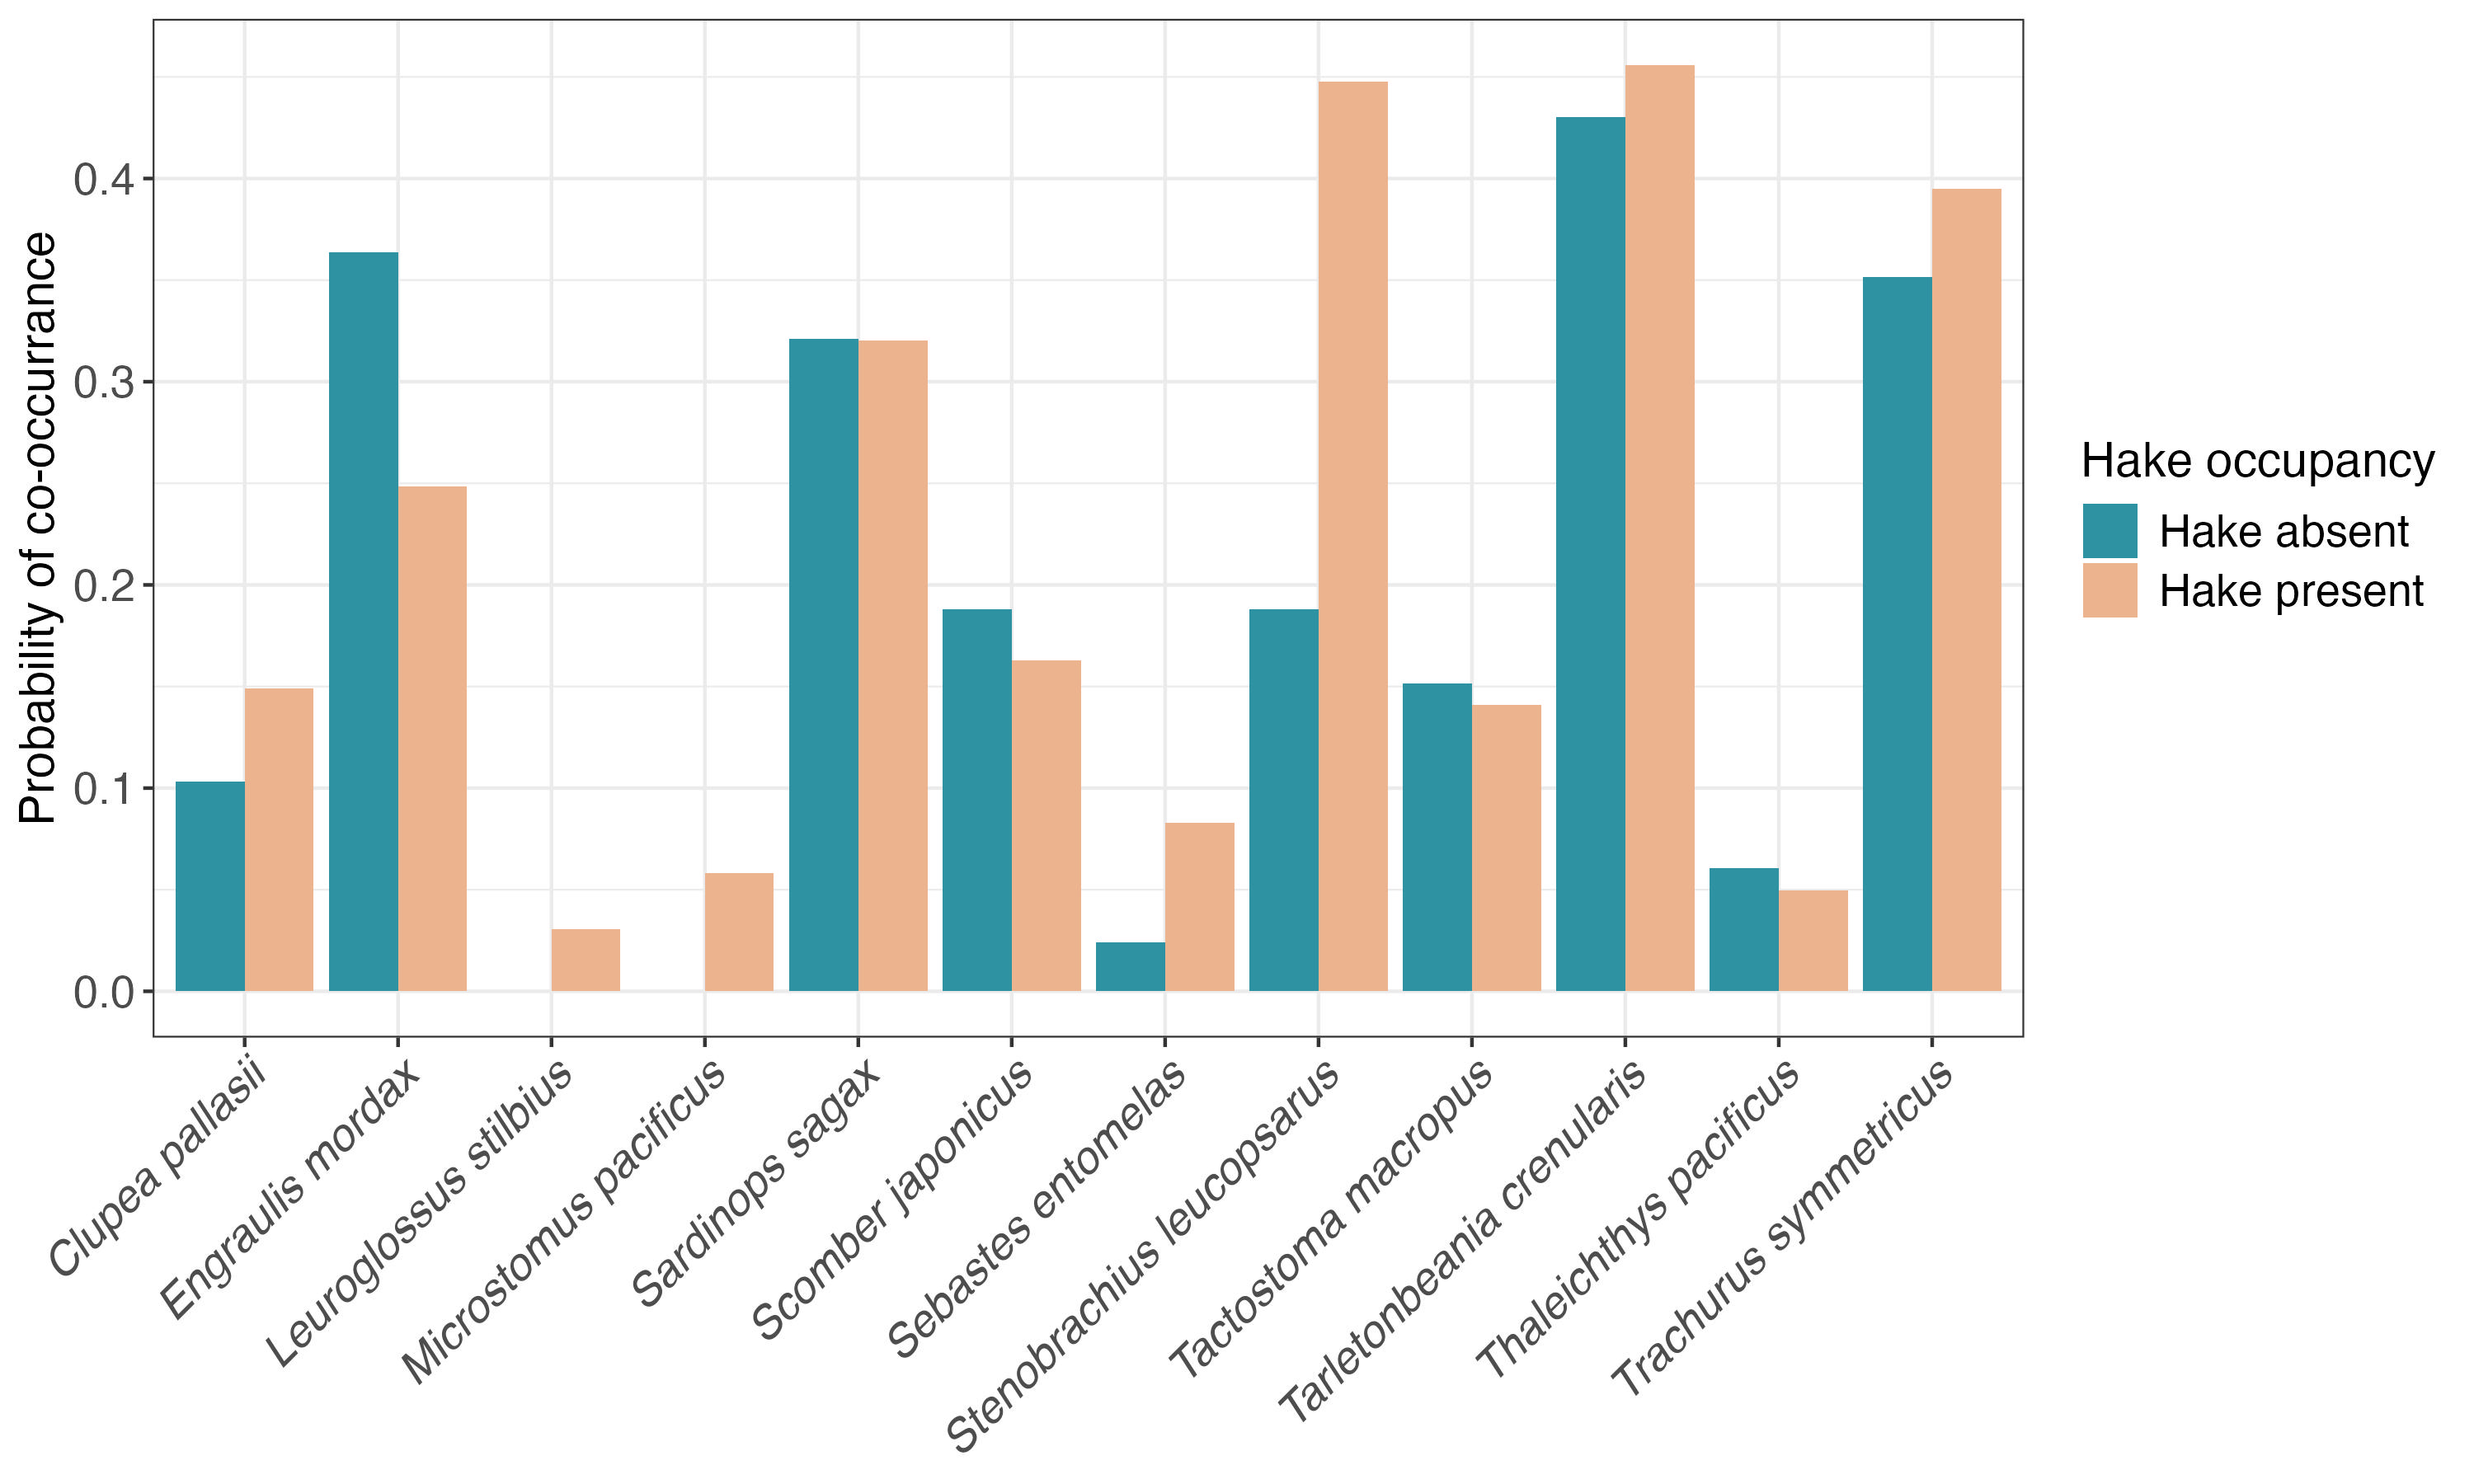
\includegraphics[width=0.99\textwidth]{plots/8_Supplementary_Figure_4.jpg}
\caption{Probability of species co-occurrence with Pacific hake, where blue bars represent non-occurrence and orange bars indicate co-occurrence. \textit{Engraulis mordax} exhibits the most inverse habitat overlap with hake, while \textit{Stenobrachius leucopsarus} shows the highest habitat overlap.}
\end{figure}

%%% Each figure should be on its own page
\begin{figure}
\centering
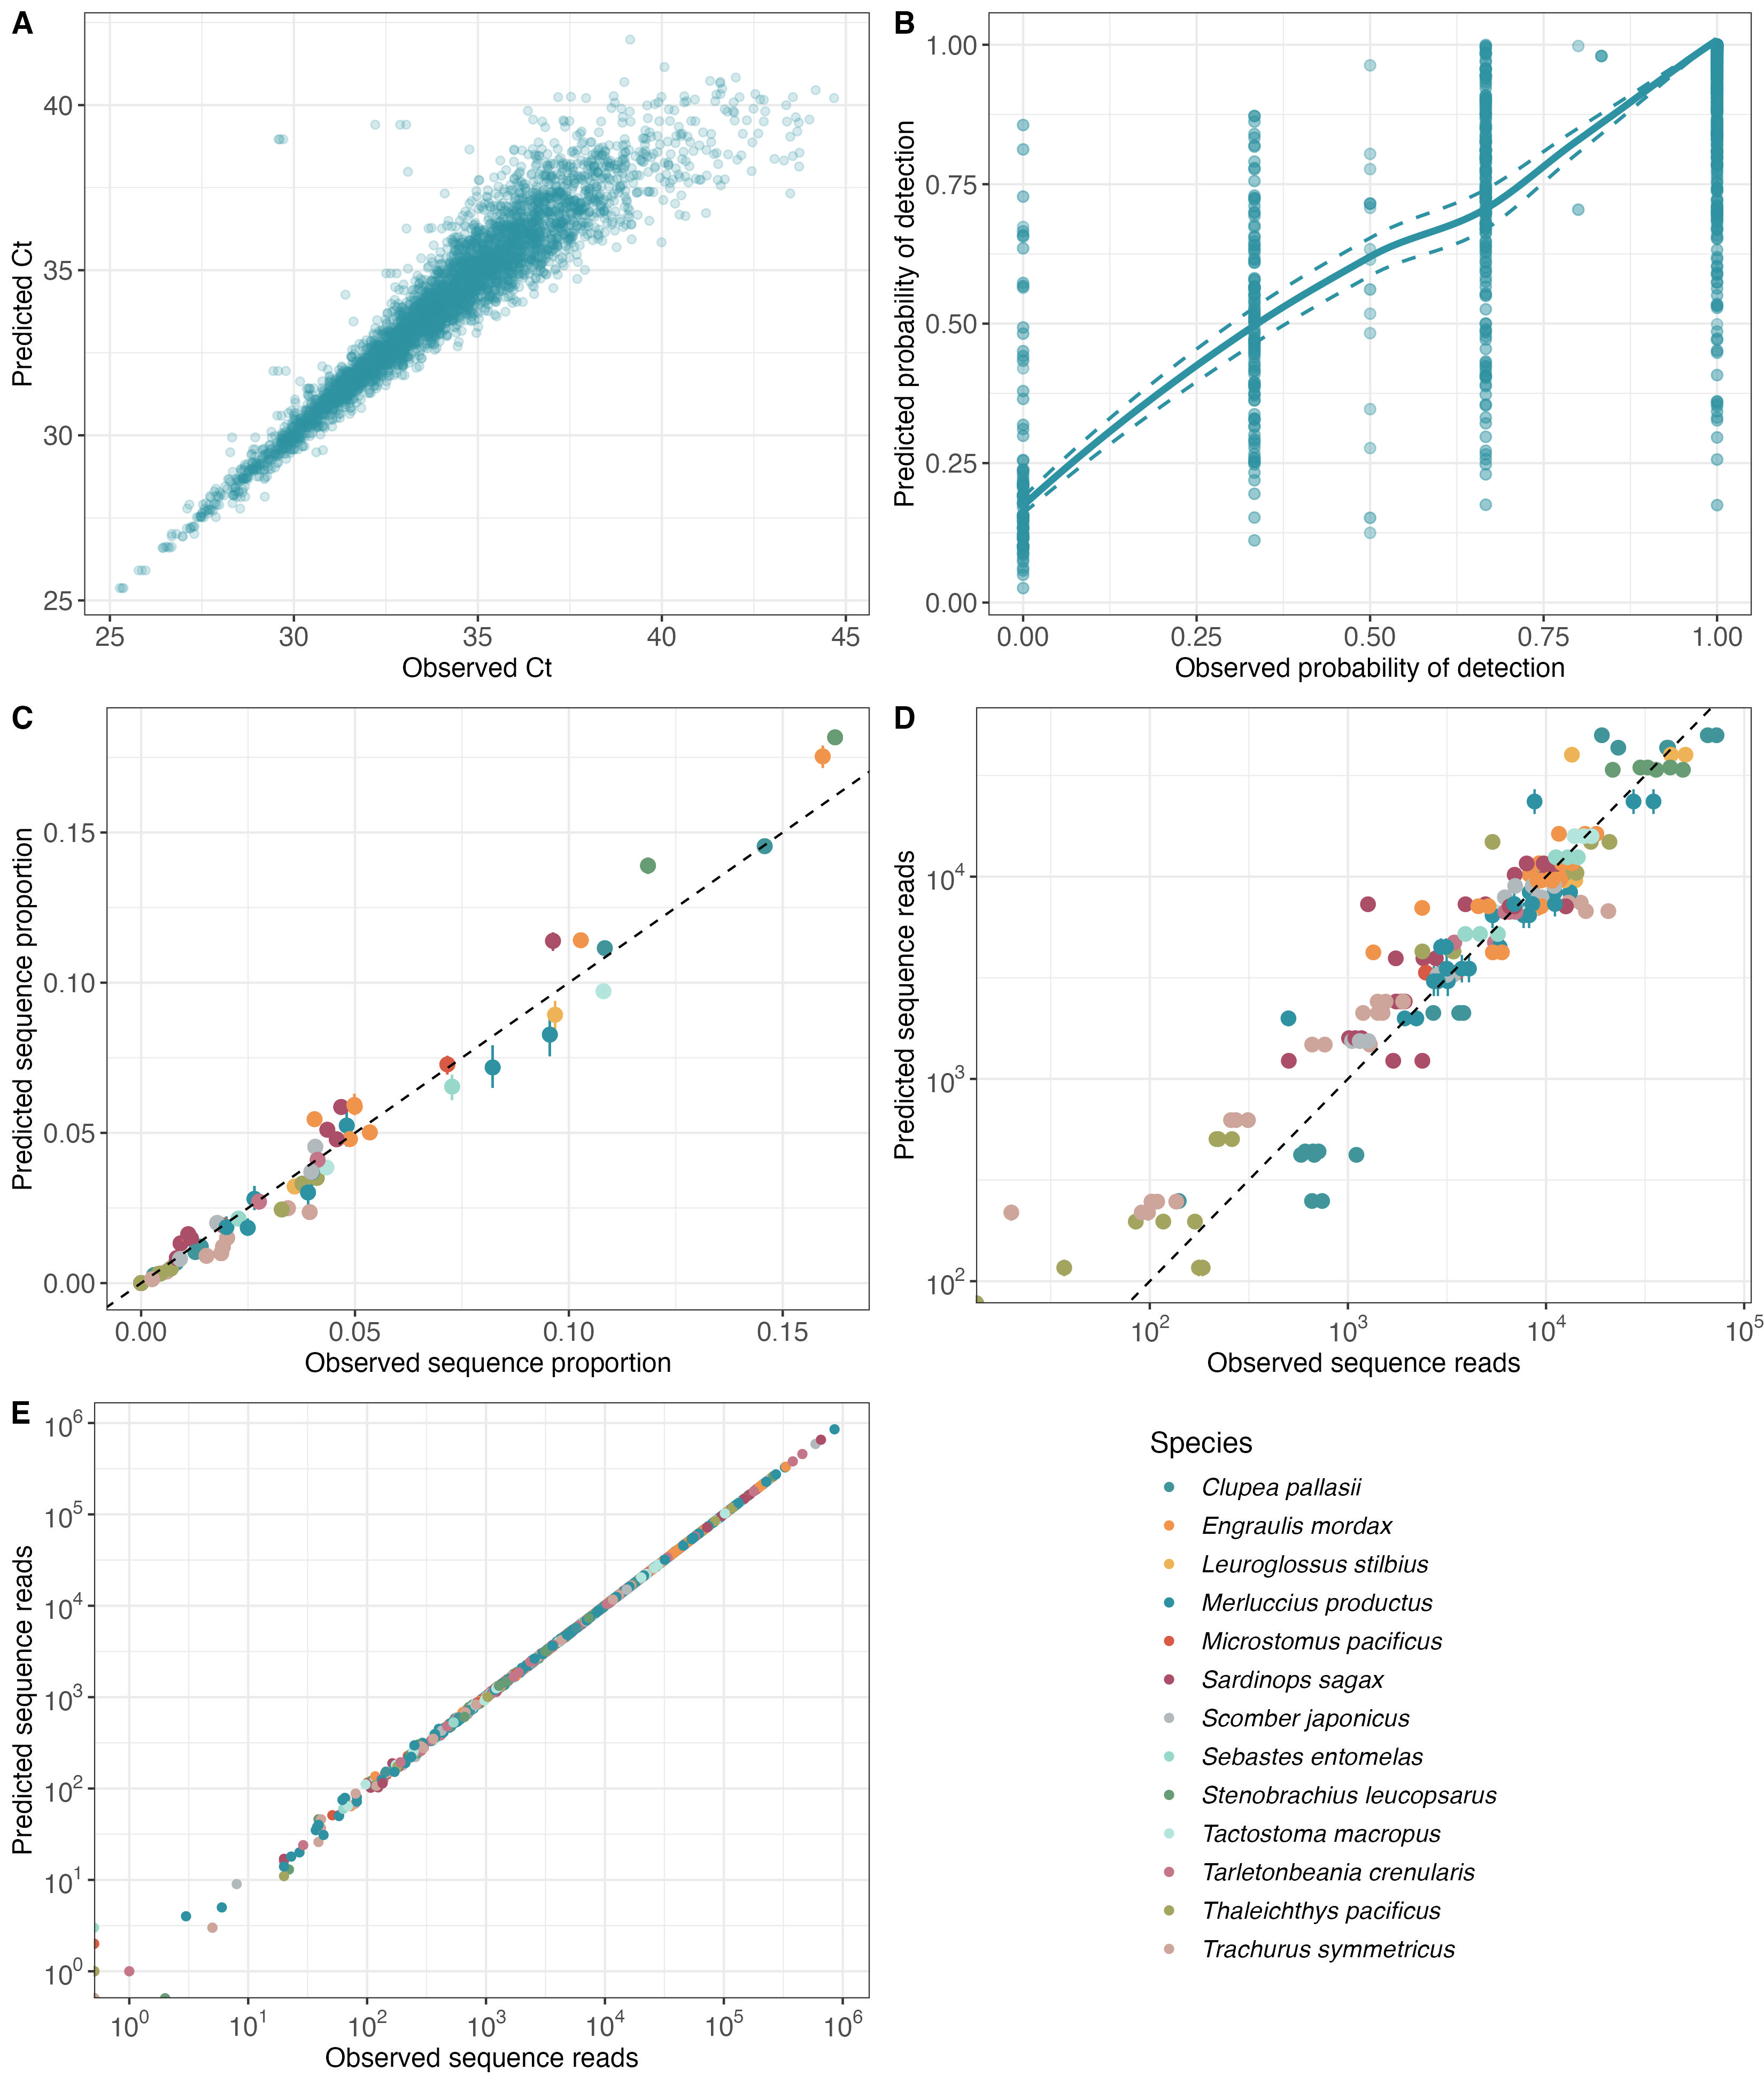
\includegraphics[width=0.98\textwidth]{plots/9_Supplementary_Figure_5.jpg}
\caption{Mean posterior predictions for three model compartments, qPCR continuous model (A), qPCR occupancy model (B), mock community model (C and D on species proportions and number of reads) and metabarcoding model (E)}
\end{figure}

%%% Each figure should be on its own page
\begin{figure}
\centering
\includegraphics[width=0.89\textwidth]{plots/10_Supplementary_Figure_6.jpg}
\caption{Estimated species eDNA concentration (copies/L) for all the species included in this study concentration across 0, 50, 150, 300, and 500m depth samples, without spatial smoothing.}
\end{figure}




\begin{table}\centering
\caption{Initial proportional abundances (measured by amplifying the 12S rRNA gene using MarVer1 primers \cite{valsecchi2020} and ddPCR QX200 Droplet Digital PCR system (Bio-Rad, Inc.)) of the selected species (n=12) across different mock communities (n=8). NA represent no DNA template included.}
    \begin{tabular}{lcccccccc}
        \toprule
        {Species} & \multicolumn{2}{c}{Mock1} & \multicolumn{2}{c}{Mock2} & \multicolumn{2}{c}{Mock3} & \multicolumn{2}{c}{Mock4} \\
        & Even & Skew & Even & Skew & Even & Skew & Even & Skew \\
        \midrule
        \textit{Clupea pallasii}           & 0.437 & 0.325  & 0.042  & 0.009     & -         & -          & 0.025      & 0.038 \\
        \textit{Engraulis mordax}          & 0.122 & 0.034  & 0.15 & 0.15       & 0.146      & 0.16       & 0.308      & 0.478 \\
        \textit{Leuroglossus stilbius}     & 0.108 & 0.29   & - & -         & -         & -         & -         & - \\    
        \textit{Merluccius productus}      & 0.079 & 0.144  & 0.12 & 0.06       & 0.117      & 0.075      & 0.247      & 0.287 \\
        \textit{Microstomus pacificus}     & -    & -     & 0.057  & 0.215     & -         & -         & -         & - \\    
        \textit{Sardinops sagax}           & 0.028 & 0.033  & 0.14 & 0.035      & 0.137      & 0.025      & 0.289      & 0.131 \\
        \textit{Scomber japonicus}         & -    & -     & 0.122  & 0.053      & 0.119      & 0.027     & -         & - \\    
        \textit{Sebastes entomelas}        & -    & -     & - & -          & 0.068      & 0.218     & -         & - \\    
        \textit{Stenobrachius leucopsarus} & -    & -     & - & -          & 0.356      & 0.487     & -         & - \\    
        \textit{Tactostoma macropus}       & -    & -     & 0.13 & 0.324     & -         & -         & -         & - \\    
        \textit{Tarletonbeania crenularis} & -    & -     & 0.083  & 0.124     & -         & -         & -         & - \\    
        \textit{Thaleichthys pacificus}    & 0.123 & 0.113  & 0.099  & 0.012     & -         & -          & 0.013      & 0.021 \\
        \textit{Trachurus symmetricus}     & 0.103 & 0.06   & 0.057  & 0.018      & 0.056      & 0.008      & 0.118      & 0.04 \\
        \bottomrule
    \end{tabular}
\end{table}

\bibliography{pnas-sample}

\end{document}
